\chapter{Locality of constraints}\label{ch:locality}

Is the topology of the history space a consequence of integer divisibility, or of the \emph{form} of the constraint? This chapter answers for one precisely stated class. A \emph{pairwise grammar} specifies, for every ordered pair of labels, whether the first may be immediately followed by the second; histories are the orderings all of whose consecutive pairs are allowed. No integers, no divisibility. For six labels we prove that such a grammar never produces a two-dimensional hole. Constraints on consecutive \emph{triples} can, and so can prefix-set constraints. The dividing line is how local the forbidden pattern is. Every statement here is for six labels; no version for other lengths is claimed.

\section{Adjacency complexes}\label{sec:adjacency}
Let $G$ be a digraph on $[6]$ and $A_G$ the set of orderings $(x_1,\dots,x_6)$ with $(x_t,x_{t+1})\in G$ for all $t$. Such $A_G$ is not prefix-defined in general. Let $B$ be the set of ordered pairs $p=(x,y)$, $x\ne y$, not in $G$; an ordering is non-admissible iff $x$ is immediately followed by $y$ for some $p\in B$. For $p=(x,y)$ let $Z_p\subseteq T$ be the subcomplex generated by the flags in which $x$ is immediately followed by $y$, and $Z_S=\bigcap_{p\in S}Z_p$. Then
\[
Y_{A_G}=\bigcup_{p\in B}Z_p .
\]
@@lem:Z+analytic@@

\section{The pairwise-adjacency theorem}
@@thm:pairwise+computer-assisted@@
The proof reduces the statement to three finite facts about the thirty ordered pairs.
@@RAW:ch14.tex::\begin{enumerate}[label=(F\arabic*)]::\end{proof}@@
The three finite facts (F1)--(F3) were verified by exact elimination over $\F$: (F1) for all $30$ pairs, (F2) for all $435$ pairs of pairs, (F3) for all $4060$ triples. Non-emptiness in (F2) and (F3) also follows from \cref{lem:Z}; (F1) and the connectedness part of (F2) are certified by computation only.

\begin{figure}[ht]\centering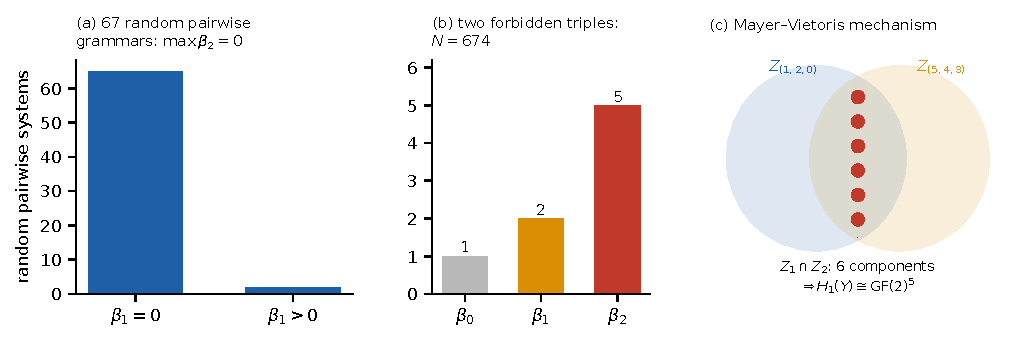
\includegraphics[width=\textwidth]{figures/fig_locality.pdf}
\caption{Pairwise versus triple-local constraints. (a)~$\max\beta_2$ over random pairwise grammars (exact; $\max=0$). (b)~Betti numbers of the system with two forbidden consecutive triples: $(1,2,5)$ with $N=674$ (exact). (c)~The Mayer--Vietoris mechanism: $Z_1\cap Z_2$ has six components, giving $H_1(Y)\cong\F^5$.}\label{fig:locality}
\end{figure}

The intersections $Z_S$ are not acyclic: for $Z_{pqr}$ there are $120$ triples with $Z_{pqr}$ disconnected, which is harmless because only the images of components under $d^1$ matter. The argument uses only the low-degree information (F1)--(F3); a proof by acyclicity of all intersections is not available.
@@cor:symbolic+analytic@@
@@obs:sym+bounded@@

\section{Sharpness: constraints on consecutive triples}
@@prop:triple+computer-assisted@@
In an exploratory sample of $19{,}993$ random systems defined by forbidding consecutive triples, $905$ had $\beta_2>0$.

\section{The locality order}
@@obs:locality@@
The pairwise theorem is not claimed for $k\ne6$: the finite lemmas (F1)--(F3) are specific to $k=6$, and the spectral-sequence argument needs their analogues at the new $k$. We have no purely local criterion for hollowness (\cref{obs:cycle-census}), and no classification of which digraph families give $\beta_1>0$.
